\documentclass[a4paper,12pt]{article}
\usepackage[utf8]{inputenc}
\usepackage[spanish]{babel}
\usepackage{color}
\usepackage{parskip}
\usepackage{graphicx}
\usepackage{multirow}
\usepackage{listings}
\usepackage{vmargin}
\usepackage{datetime}
\usepackage{float}
\newdate{date}{31}{08}{2017}
\graphicspath{ {imagenes/} }
\definecolor{mygreen}{rgb}{0,0.6,0}
\definecolor{lbcolor}{rgb}{0.9,0.9,0.9}
\usepackage{epstopdf}


\setpapersize{A4}
\setmargins{2.5cm}       % margen izquierdo
{1.5cm}                        % margen superior
{16.5cm}                      % anchura del texto
{23.42cm}                    % altura del texto
{10pt}                           % altura de los encabezados
{1cm}                           % espacio entre el texto y los encabezados
{0pt}                             % altura del pie de página
{2cm}     


\begin{document}
\title{Tarea de Teoría 1}
\author{
Christofer Fabián Chávez Carazas \\
\small{Universidad Nacional de San Agustín de Arequipa} \\
\small{Escuela Profesional de Ciencia de la Computación} \\
\small{Computación Centrada en Redes}
}
\date{\displaydate{date}}

\maketitle

\begin{enumerate}
  \item \textbf{Codificar la secuencia 10110110:}
  \begin{figure}[H]
   \centering
   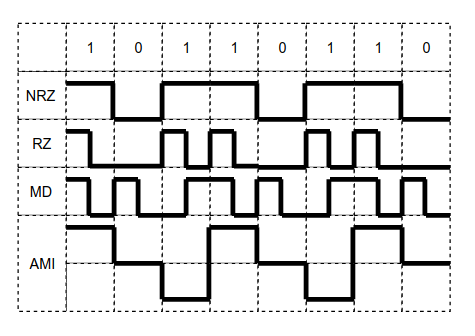
\includegraphics[scale = 0.6]{1.png}
  \end{figure}
  
  \item \textbf{Sea una transmisión asíncrona por una línea de comunicación, la velocidad de transmisión en los dos
  canales es de 19200 bps. Cada carácter enviado consta de 8 bits de datos, 2 bit de start y 1 bit de stop y
  cada carácter debe estar precedido de un silencio de transmisión de 2 mseg.}
  \begin{itemize}
   \item \textbf{Calcular el rendimiento (porcentaje de información útil transmitida, con respecto a la información total transmitida)}
   $$Rendimiento\:=\frac{8\: bits\:de\:datos}{8 + 2 + 1\: bits\:totales}= \:\frac{8}{11}=0.72 = 72\%$$
   \item \textbf{¿Cuánto demorará en transmitir un archivo de 100K bytes de información?}
   $$100K = 1024 * 8 * 100 = 819200\: bits$$
   $$819200/19200 = 42.66\:s$$
   $$819200/11 = 74473\:paquetitos$$
   $$74473 * 0.002 = 148.946\:s$$
   $$Total = 42.66 + 148.946 = 191.606\:s$$
  \end{itemize}
  
  \item \textbf{Responder:}
  \begin{itemize}
   \item \textbf{¿Cuál es el rendimiento de una transmisión serie asíncrona de 9600 bps con 8 bits de datos, 1 bit de
start y 1 bit de stop?}
  $$Rendimiento=\frac{8\:bits\:de\:datos}{8 + 1 + 1\:bits\:totales} = \frac{8}{10} = 0.80 = 80\:\%$$

   \item \textbf{¿Cuanta información se transmite en un día si entre carácter y carácter debe haber
1 mseg de silencio?}
  $$24\:h = 86400\:s$$
  $$9600\:bps / 10 = 96\:paquetitos * 0.001 = 0.096 + 1\:s = 1.096\:$$
  $$86400 / 1.096 = 78833 * 96 = 756968 * 10 = 75679680\:bits = 9.0217\:M$$
  \end{itemize}
  
  \item \textbf{¿Cuáles y como son los puertos seriales y paralelos presentes en una computadora? Hacer la
descripción física y funcional.}

  Los puertos seriales que comúnmente se utilizan son el DB25S  de 25 pines y DB9S de 9 pines:
  \begin{figure}[H]
   \centering
   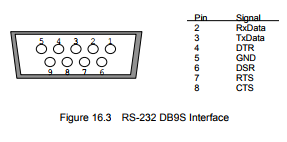
\includegraphics[scale = 0.4]{2.png}
  \end{figure}
  \begin{figure}[H]
   \centering
   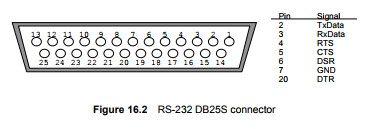
\includegraphics[scale = 0.4]{3.png}
  \end{figure}
  Los tipos de señales especificados en el estándar son los siguientes:
  \begin{itemize}
   \item \textbf{Masa:} GND para aislamiento del conector con enlace al chasis de la terminal; SG Señal sobre la que se establece la tensión de las demás señales del conector
   \item \textbf{Canal Principal:} Conjunto de señales de datos y control, TxD y RxD líneas de transmisión y recepción 
   respectivamente; RTS, CTS, DSR y DCD señales básicas, DTR y RI señales conmutadas y SQ, CH y CI señales de calidad y canales.
   \item \textbf{Transmisión Síncrona:}  DA, DD y DB exclusivas de sincronía.
   \item \textbf{Canal Secundario:} para algunos modelos DCE.
   \item \textbf{Terminales sin Asignación Fija.}
  \end{itemize}
  Los puertos paralelos que comúnmente se utilizan son el tradicional tipo D de 25 pines llamado IEEE 1284-A, el tradicional
  conector \textit{Centronics} llamado IEEE 1284-B y un nuevo conector más pequeño similar al \textit{Centronics} es llamado IEEE
  1284-C.
  \begin{figure}[H]
   \centering
   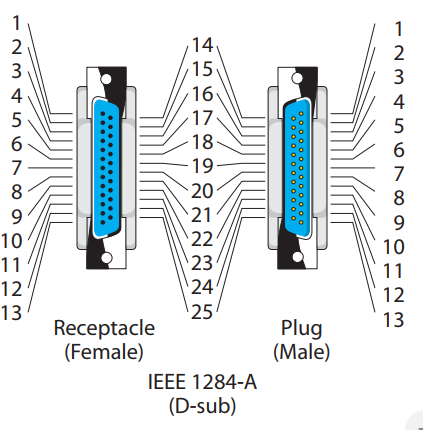
\includegraphics[scale = 0.4]{4.png}
  \end{figure}
  \begin{figure}[H]
   \centering
   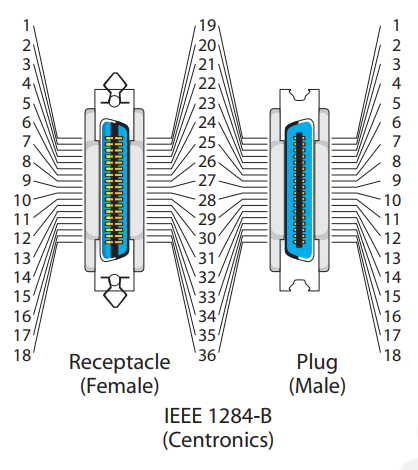
\includegraphics[scale = 0.4]{5.png}
  \end{figure}
  \begin{figure}[H]
   \centering
   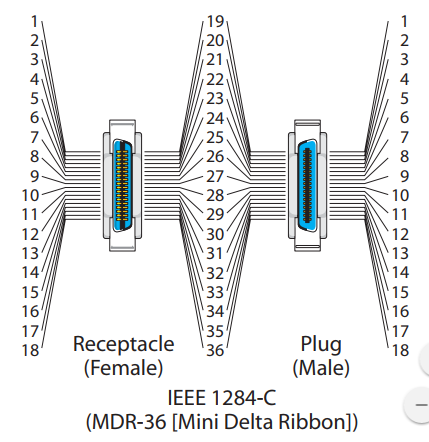
\includegraphics[scale = 0.4]{6.png}
  \end{figure}
  Para estos puertos existen varios modos:
  \begin{itemize}
  \item \textbf{Modo de Compatibilidad:} Básicamente en este modo se mueven datos desde una PC hacia
  un periférico como una impresora. Se pueden mover hasta 8 bits de datos al mismo tiempo.
  \item \textbf{Modo Nibble:} Es lo contrario al modo anterior; se mueven datos desde el periférico hacia la PC.
  Se pueden mover hasta un nibble de información (4 bits).
  \item \textbf{Modo Byte:} Es igual que el modo nibble solo que ahora se puede mover
  hasta un byte de información.
  \item \textbf{Modo EPP:} Este modo funciona de forma bidireccional.
  \end{itemize}

  \item \textbf{¿Cómo es el manejo de errores en la transmisión síncrona?}  
  Un error ocurre cuando un bit es alterado durante la transmisión y recepción. Existen dos tipos de errores: Un bit simple, cuando
  el error ocurre con un solo bit y no afecta a los otros, y el error en ráfaga, cuando más de un bit está comprometido.
  Para una transmisión síncrona existen dos tipos de algoritmos para la detección de errores:
  \begin{itemize}
   \item \textbf{Comprobación de Paridad:} Consiste en añadir un bit de paridad al final del bloque de datos. El valor de este bit se determina de tal forma que el
   carácter resultante tenga un número impar de unos (paridad impar) o un número par (paridad par). La utilización de bits de paridad no es infalible, ya que
   los impulsos de ruido son a veces lo suficientemente largos como para destruir más de un bit, especialmente a velocidades de transmisión altas.
   \item \textbf{Comprobación de Redundancia Cíclica:} Dado un bloque o mensaje de $k-bits$, el transmisor genera una secuencia de $nbits$, denomidanda
   secuencia de comprobación de la trama, de tal manera que la trama resultante, con $n + k bits$, sea divisible por algún número predeterminado.
   El receptor entonces dividirá la trama recibida por ese número y, si no hay resto en la división, se supone que no ha habido errores.
  \end{itemize}

 
  \item \textbf{¿Cómo es el manejo de errores en la transmisión asíncrona?}\\
  En la transmisión asíncrona se envía bits de comienzo, bits de datos y bits de parada. Los bits de datos, al igual que la transmisión síncrona,
  van seguidos de un bit de paridad, que ocupará por tanto la posición del bit más significativo. Este bit es generado de la misma forma explicada en la pregunta anterior.
  
  \item \textbf{Describir las características y diferencias entre RDSI, DSL y ADSL}
  \begin{itemize}
   \item \textbf{RDSI}
   
   La red Digital de Servicios Integrados para cualquier tipo de información
   (voz, datos, imágenes, etc.), permite una vez codificado digitalmente tratar
   la información de idéntica manera, con la única diferencia de las
   velocidades requeridas.
   Una RDSI tiene las siguientes características:
   \begin{itemize}
    \item Soporte de aplicaciones: Soporta tanto voz como datos, utilizando un
    conjunto de aplicaciones estándar.
    \item Soporte para aplicaciones conmutadas y no conmutadas: RDSI
    admite tanto conmutación de circuitos como de paquetes. Además, RDSI
    proporciona servicios no conmutados con líneas dedicadas a ello.
    \item Dependencia de conexiones de 64 kbps: RDSI proporciona
    conexiones de conmutación de circuitos y de conmutación de paquetes a 64
    Kb/s. Este es el bloque de construcción fundamental de la RDSI.
    \item Inteligencia en la red: Se espera que la RDSI pueda proporcionar
    servicios sofisticados por encima de la sencilla situación de una llamada de
    circuito conmutado.
    \item Arquitectura de protocolo en capas: Los protocolos para acceso a la
    RDSI presentan una arquitectura de capas que se puede hacer corresponder
    con la del modelo OSI.
    \item Variedad de configuraciones: Es posible más de una configuración
    física para implementar RDSI. Esto permite diferencias en políticas
    nacionales, en el estado de la tecnología, y en las necesidades y equipos
    existentes de la base de clientes.
   \end{itemize}
   
   \item \textbf{DSL}
   
   La tecnología DSL(Línea de Abonado Digital) explota la red de acceso de cobre existente, a la que incorpora los equipos
   correspondientes en ambos extremos con lo que se consigue transformar la línea telefónica en
   un vínculo de transmisión de datos de alta velocidad. DSL posibilita la capacidad de transformar casi
   700 millones de líneas telefónicas instaladas por todo el mundo en autopistas de datos capaces
   de transportar voz y datos digitales a hogares y negocios. Todas las tecnologías DSL se han beneficiado de
   los avances en la electrónica (aumento de potencia de procesamiento, reducción en el consumo de energía, etc).
   Aparte de mejoras en la funcionalidad, los módems DSL emplean técnicas más sofisticadas de modulación y de
   codificación, y el uso de chips genera una baja de los costos y un consumo de energía reducido.
   
   \newpage
   
   \item \textbf{ADSL}
   
   ASDL (\textit{Asymmetric Digital Subscreiber Line}) es una técnica de datos a gran velocidad sobre el par de cobre.
   Esta técnica es implementada por muchas empresas telefónicas que ya contaban con el tendido de cables de cobre, con el fin de ocupar
   un margen de frecuencias mucho más amplio que va desde los 24 KHz hasta los 1104 KHz, aproximadamente, permitiendo el
   uso simultáneo de canales de voz y datos, pero se necesita que en la central se separen las señales y cada una sea derivada a la
   red correspondiente. \\
   Al tratarse de una modulación asimétrica, el módem ADSL situado en el extremo del usuario es distinto del ubicado al otro del lazo, en la central local.
   El splitter no es más que un conjunto de dos filtros: uno paso alto y otro paso bajo. La finalidad de estos filtros es la de separar las señales
   transmitidas, o sea, las señales de baja frecuencia y las de alta frecuencia.
  \end{itemize}

  
  
  \item \textbf{Defina al menos dos sistemas comerciales que usen conexión simplex, semiduplex y fullduplex.}
  
  \begin{itemize}
   \item \textbf{Simplex:} La transmisión simplex (sx) o unidireccional es aquella que ocurre en una dirección solamente, deshabilitando al receptor de responder al transmisor. Normalmente la transmisión simplex no se utiliza donde se requiere interacción humano-máquina.
   Ejemplos de transmisión simplex son: La radiodifusión (broadcast) de TV y radio.
   \item \textbf{SemiDuplex:} Permite transmitir en ambas direcciones; sin embargo, la transmisión puede ocurrir solamente en una dirección a la vez. Tanto transmisor y receptor comparten una sola frecuencia. Un ejemplo típico de semiduplex es el radio de banda civil (CB) donde el operador puede transmitir o recibir, no pero puede realizar ambas funciones simultáneamente por el mismo canal.
   \item \textbf{Fullduplex:} Permite transmitir en ambas dirección, pero simultáneamente por el mismo canal. Existen dos frecuencias una para transmitir y otra para recibir. Ejemplos de este tipo abundan en el terreno de las telecomunicaciones, el caso más típico es la telefonía, donde el transmisor y el receptor se comunican simultáneamente utilizando el mismo canal, pero usando dos frecuencias. 
  \end{itemize}

\begin{thebibliography}{1}

\bibitem{book}
Stallings, William. ``Data and computer communications.'' Prentice Hall (2005).

\bibitem{my}
Chávez, Christofer. ``Cuestionario Previo de la Primera Práctica.'' (2017).

\end{thebibliography}
  
\end{enumerate}


\end{document}

